\section{Training and Sampling}\label{sec:vaepp}
In this section, we will propose two training methods and a sampling method for VAEPP. The main difference between these two trainings method is the training method of the discriminator. 

\subsection{Naive training for VAEPP} \label{subsec:naive_vaepp}
By \cref{subsec:inference}, an approximation discriminator is trained by:
\begin{equation*}
	W^1(p^\dag, p^*) = \sup_{Lip(D) \leq 1} \E_{p^\dag} D(x) - \E_{p^*} D(x)
\end{equation*} 
where $p^\dag(x) = \E_{p_\mathcal{N}(z)} p_\theta(x|z)$. The real discriminator should be obtained by $W^1(p_\theta, p^*)$, but it is expensive to sample from $p_\theta$ in training and then $W^1(p^\dag, p^*)$ is used to obtain an approximation discriminator. As the result, the approximation discriminator may be invalid when $p_\lambda$ is too far from $p_\mathcal{N}$, \IE $\beta$ is too large. Fortunately, the training for $\beta$ can avoid this: when $\beta$ becomes too large and $D$ becomes invalid, ELBO will be worse and then $\beta$ will decrease. The other parameters is trained by SGVB:
\begin{equation*}
	\max_{\theta, \phi, \beta} \mathcal{L}(\theta, \phi, \beta, \omega)
\end{equation*}
Above two training process run alternatively, which is called the naive training algorithm for VAEPP, in \cref{alg:vaepp},. 
\begin{algorithm}[tb]
\caption{The naive training algorithm for VAEPP}
\label{alg:vaepp}
\textbf{Require}: The gradient penalty algorithm $R$, the batch size $b$, the number of critic iterations per generator iteration $n_c$, the parameters for Adam Optimizers, $\tau$. 

\begin{algorithmic}[1] %[1] enables line numbers
\WHILE{$\theta, \phi, \beta, \omega$ have not converged}
\FOR {$k = 1, \ldots n_c$}
\FOR {$i = 1, \ldots, b$}
\STATE Sample $e, x \sim p^*$, $z \sim q_\phi(z|e)$, $\epsilon \sim p_\mathcal{N}$
\STATE $Z^{(i)} \gets \frac{1}{2}(e^{-\beta D(G(\epsilon))} + \frac{f_\lambda(z)}{\hat{q}_\phi(z)})$
\STATE $\mathcal{L}^{(i)} \gets \ln p_\theta(x|z) + \ln f_\lambda(z) - \ln q_\phi(z|e)$
\ENDFOR
\STATE $\mathcal{L} \gets \frac{1}{b}\sum_{i}^b \mathcal{L}^{(i)} - \ln (\frac{1}{b}\sum_{i}^b Z^{(i)})$
\STATE $\theta, \phi, \beta \gets $ Adam $(\nabla_{\theta, \phi, \beta} \mathcal{L}, \{\theta, \phi, \beta\}, \tau)$
\ENDFOR
\FOR {$i = 1, \ldots, b$}
\STATE Sample $e, x \sim p^*$, latent variable $z \sim p_\mathcal{N}$
\STATE	$\hat{e} = G(z)$, get gradient penalty $\zeta \gets R(e, \hat{e})$
\STATE $L^{(i)} \gets D(\hat{x}) - D(x) + \zeta$
\ENDFOR
\STATE $\omega \gets $ Adam $(\nabla_{\omega} \frac{1}{b}\sum_{i}^b L^{(i)}, \omega, \tau)$
\ENDWHILE
\end{algorithmic}
\end{algorithm}

\subsection{Combing training for VAEPP} \label{subsec:improve_of_vaepp}

\begin{figure}[tb]
	\centering
	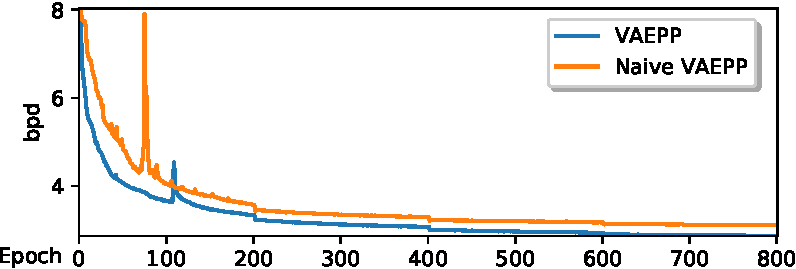
\includegraphics[width=0.9\columnwidth]{../dist.strip/loss_curves}
	\caption{
	Training loss of Naive VAEPP and VAEPP on CIFAR-10. Naive VAEPP is more unstable and nearly crashes at 80 epoch while VAEPP has a little acceptable gap. From global view, the training loss of VAEPP is more smooth than Naive VAEPP and is better than Naive VAEPP's over almost all training process, which validates the motivation in \cref{subsec:improve_of_vaepp}. There are little gaps at per 200 epoch because learning rate is reduced to half at every 200 epoch. 
	}
	\label{fig:loss_curves}
\end{figure}

However, the training process of \cref{alg:vaepp} is unstable and inefficient, as shown in \cref{fig:loss_curves}. 
We suspect that the two independent optimizations instead of one whole optimization, may lower the log-likelihood and stability. Therefore, we try to combine the training for $\theta, \phi, \beta, \omega$ into a whole optimization. 
Our solution is to use SGVB with gradient penalty regularizer to train VAEPP:
\begin{equation*}
	\max_{\theta, \phi, \beta} \max_{Lip(D) \leq 1} \mathcal{L}(\theta, \phi, \beta, \omega) 
\end{equation*} 
In such optimization, the behavior of $\theta, \phi, \beta$ is same as \cref{alg:vaepp} since the optimization for them is same. For $\omega$, 
$\max_{Lip(D) \leq 1} \mathcal{L}(\theta, \phi, \beta, \omega)$ indeed finds a suboptimal discriminator in $W^1(p^\dag, p^*)$ (sign $\simeq$ means that optimizations at left and right are equivalent):
\begin{align*}\label{eq:improve_vaepp}
	&\max_{Lip(D) \leq 1} \mathcal{L} \simeq \max_{Lip(D) \leq 1} \{ -\E_{q_\phi(z)} \beta*D(G(z)) - \ln Z \}\\ 
	&\leq \beta \max_{Lip(D) \leq 1} \{ \E_{p_\mathcal{N}(z)} D(G(z)) - E_{q_\phi(z)} D(G(z)) \} \tag{9} \\
	&= \beta W^1(p^\dag, p_r) \approx \beta W^1(p^\dag, p^*) 
\end{align*}
where $p_r$ denotes $p_r(x) = \E_{q_\phi(z)} p_\theta(x|z)$, consisting of reconstructed data. 
The last approximation sign is from the fact that $p_r \rightarrow p^*$ after  few epochs in training of VAE. \cref{eq:improve_vaepp} also uses the assumption $D(G(z)) = \E_{p_\theta(x|z)} D(x)$ introduced in \cref{subsec:inference} to simplify equation. The inequality of $\ln Z$ is:
\begin{equation*}
	\ln Z = \ln \E_{p_\mathcal{N}(z)} e^{- \beta * D(G(z))} \geq \E_{p_\mathcal{N}(z)} [- \beta * D(G(z))]
\end{equation*}

\cref{eq:improve_vaepp} indicates that it is reasonable to obtain a suboptimal discriminator $D$ by optimizing $\mathcal{L}$ with the gradient penalty term, and the gradient penalty term should be multiplied by $\beta$. In this way, the optimizations for $\theta, \phi, \beta$ and $\omega$ are combined into one, as shown in \cref{alg:improved_vaepp}. 
Moreover, the discriminator trained by \cref{alg:vaepp} and in \cref{alg:improved_vaepp}, are both approximations to the real discriminator in $W^1(p_\theta, p^*)$. 

Thanks to the gradient penalty terms provided by WGAN-GP and WGAN-div, we enjoy stable and efficient training. The model trained by \cref{alg:vaepp} is called Naive VAEPP and the model trained by \cref{alg:improved_vaepp} is called VAEPP. 
\begin{algorithm}[tb]
\caption{The combing training algorithm for VAEPP}
\label{alg:improved_vaepp}
\textbf{Require}: The gradient penalty algorithm $R$, the batch size $b$, the parameters for Adam Optimizers, $\tau$. 

\begin{algorithmic}[1] %[1] enables line numbers
\WHILE{$\theta, \phi, \beta, \omega$ have not converged}
\FOR {$i = 1, \ldots, b$}
\STATE Sample $e, x \sim p^*$, $z \sim q_\phi(z|e)$, $\epsilon \sim p_\mathcal{N}$
\STATE $\hat{e} = G(\epsilon)$, get gradient penalty $\zeta \gets R(e, \hat{e})$ 
\STATE $Z^{(i)} \gets \frac{1}{2}(e^{-\beta D(G(\epsilon))} + \frac{f_\lambda(z)}{\hat{q}_\phi(z)})$
\STATE $\mathcal{L}^{(i)} \gets \ln p_\theta(x|z) + \ln f_\lambda(z) - \ln q_\phi(z|e) + \beta \zeta$
\ENDFOR
\STATE $\mathcal{L} \gets \frac{1}{b}\sum_{i}^b \mathcal{L}^{(i)} - \ln (\frac{1}{b}\sum_{i}^b Z^{(i)})$
\STATE $\theta, \phi, \beta, \omega \gets $ Adam $(\nabla_{\theta, \phi, \beta} \mathcal{L}, \{\theta, \phi, \beta, \omega\}, \tau)$
\ENDWHILE
\end{algorithmic}
\end{algorithm}

\subsection{Sampling from VAEPP}
We apply Langevin Dynamics to sample $z$ from $p_\lambda(z)$. It could generate natural and sharp images and only requires that $\nabla_z \log p_\lambda(z)$ is computable and $p_\lambda(z_0)$ is high enough where $z_0$ is the initial point of Langevin Dynamics~\cite{song2019generative}. 
Moreover, MEG~\cite{kumar2019maximum} has implemented a Metropolis-Adjusted Langevin Algorithm (MALA) for sampling, where the formula of density also contains a discriminator term. 
But how to obtain the initial $z_0$ whose density is high enough is still a problem. 

Following the philosophy of VAEPP, \IE using the technique of GANs to assist VAEs, it is natural to use a GAN to model the distribution $q_\phi(z)$, and use samples of the GAN as the initial $z_0$ for MALA. 

The sampling of VAEPP consists of 3 parts: 
\begin{enumerate}
	\item generate initial $z_0$ by a GAN modeling $q_\phi(z)$
	\item generate $z \sim p_\lambda(z)$ from initial $z_0$ by MALA
	\item generate image from $z$ with a decoder
\end{enumerate}

This sampling process is similar to 2-Stage VAE~\cite{dai2019diagnosing}. The main difference between them is that VAEPP applies Langevin Dynamics to sample from the explicit prior but 2-Stage VAE doesn't, since the prior of 2-Stage VAE is implicit. In experiments, we found that sampling from the explicit learnable prior might improve the quality of sampling in some datasets. 

%It is hard to sample $z$ from $p_\lambda(z)$ since it is complicated. 
Accept/Reject Sampling (ARS)~\cite{bauer2019resampled} is useless for $p_\lambda$ because ARS requires that $p_\lambda(z) / p_\mathcal{N}(z)$ is bounded by a constant $M$, such that a sample could be sampled in $M$ times. It means $\beta$ is nearly 0, but not in fact.
 
 